\documentclass[lipt]{Article}
\chapter{Mengenal Python dan Anaconda}
\bootitle {by 1174086 Tia Nur Candida D4 TI 2C} 

\begin{document}
\section{Sejarah}
Python dirancang oleh Guido van Rossum yang dirilis perdana pada tahun 1991. Python diciptakan oleh Guido van Rossum pertama kali di Scitchting Mathematisch Centrum (CWI) di Belanda. Bahasa python terinspirasi dari bahasa pemrograman ABC. Pada tahun 1995, python dikembangkan oleh Guido di Corporation for National Research Initiative (CNRI) di Virginia Amerika merilis beberapa versi dari python. Penamaan Python diambil dari komedi Inggris,  Guido menamai python karena ia penggemar grup komedi Inggris bernama Monty Python. Ia kemudian menamai bahasa ciptaannya dengan nama Python.
Semua versi python dirilis bersifat open source. Hampir semua rilisan python menggunakan lisensi GFL-compatible. Berikut adalah versi python dan tanggal rilisnya ; Python 1.0 – Januari 1994, Python 1.2 – 10 April 1995, Python 1.3 – 12 Oktober 1995, Python 1.4 – 25 Oktober 1996, Python 1.5 – 31 Desember 1997, Python 1.6 – 5 September 2000, Python 2.0 – 16 Oktober 2000, Python 2.1 – 17 April 2001, Python 2.2 – 21 Desember 2001, Python 2.3 – 29 Juli 2003, Python 2.4 – 30 Nopember 2004, Python 2.5 – 19 September 2006, Python 2.6 – 1 Oktober 2008, Python 2.7 – 3 Juli 2010, Python 3.0 – 3 Desember 2008, Python 3.1 – 27 Juni 2009, Python 3.2 – 20 Februari 2011, Python 3.3 – 29 September 2012, Python 3.4 – 16 Maret 2014, Python 3.5 – 13 September 2015, Python 3.6 – 23 Desember 2016,  dan versi terbaru yaitu Python 3.7 – 27 Juni 2018. 

\section{Perbedaan Python 2 dan 3}
Python 3 lebih banyak fitur dibandingkan Python 2
Untuk membuka Python 2 hanya menggunakan perintah python saja, sedangkan Python 3 menggunakan perintah python3.

Pada source code
source code python 2 :
print "Hello world, python"
Source code python 3 :
print ("Hello world, python")

Pada python 2 didukung oleh adanya PEP (Python Enchanchement Proposal), dilengkapi dengan fitur programatikal seperti cycle detecting garbage collector untuk mengotomasi manajemen memori.
Pada python 3 memiliki kerapihan pada codebase dan menghapus redudansi juga memiliki banyak library.

\section{Implementasi}
\begin{enumerate}
\item
Google adalah perusahaan besar yang menggunakan banyak kode Python di dalam mesin pencarinya. Dan mesin pencari google adalah yang paling terkenal di dunia.
\item
Youtube, situs video terbesar dan terpopuler di dunia, sebagian besar kodenya ditulis dalam bahasa Python.
\item
Facebook, media sosial terbesar di dunia, menggunakan Tornado, sebuah framework Python untuk menampilkan timeline.
\item
Instagram, siapa yang tidak kenal. Instagram menggunakan Django, framework python sebagai mesin pengolah sisi server dari aplikasinya.
\item
Pinterest, banyak menggunakan python untuk membangun aplikasinya.
\item
Dropbox, barangkali Anda adalah salah seorang pengguna layanan ini. Dropbox menggunakan python baik di sisi server maupun di sisi pengguna layanannya.
\item
Quora, salah satu situs tanya jawab terbesar di dunia, dibangun menggunakan Python.
\item
NASA, badan antariksa Amerika ini menggunakan Python untuk bidang sainsnya.
\item
NSA, badan mata – mata Amerika banyak menggunakan Python untuk analisa kriptografi dan intelijen.
\item
Industrial Light & Magic, Pixar, banyak menggunakan Python dalam animasi movie.
\item
Blender, Maya, software pembuat animasi 3D terkenal, menggunakan Python sebagai salah satu bahasa skrip pemrogramannya.
\item
Raspberry Pi, komputer mini yang banyak digunakan sebagai mikrokontroller, menggunakan Python sebagai bahasa utamanya.
\item
ESRI, produsen terkenal pembuat software pemetaan GIS banyak menggunakan Python di produknya.
\end{enumerate}

\section{Instalasi}
\subsection{Python}
\begin{enumerate}
\item
Buka file instalasi Python, lalu run kemudian ceklis Add Python 3.7 to PATH lalu klik instal.
\begin{figure}[!htbp]
\centering
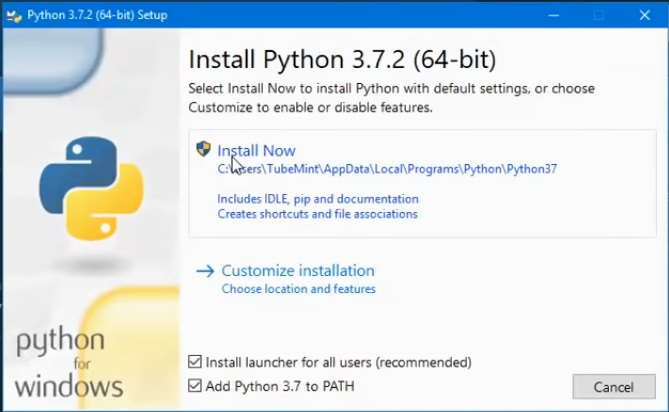
\includegraphics{start.jpg}
\caption{ Start }
\label{start}
\end{figure}
\item
Tunggu hingga proses instalasi selesai.
\begin{figure}[!htbp]
\centering
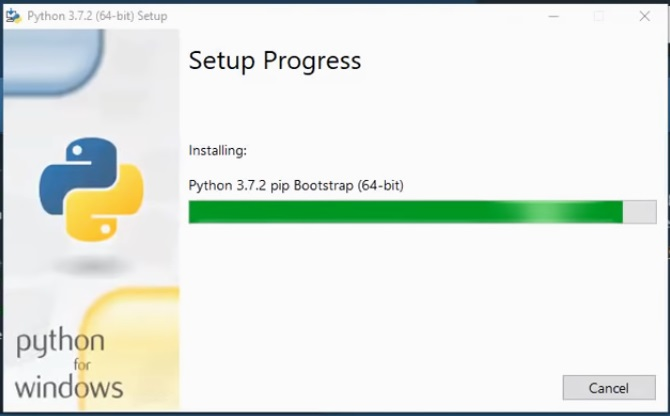
\includegraphics{process.jpg}
\caption{Process}
\label{proses}
\end{figure}
\item
Setelah instalasi selesai maka langsung close.
\begin{figure}[!htbp]
\centering
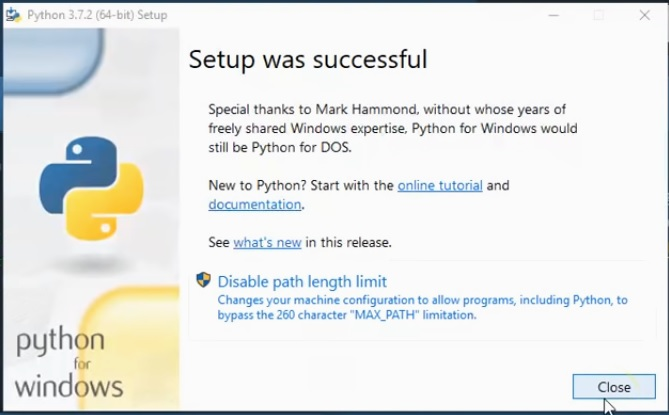
\includegraphics{finish.jpg}
\caption{Finish}
\label{finish}
\end{figure}

\end{enumerate}
\subsection{Anaconda}
\begin{enumerate}
\item 
Buka Instalasi Anaconda, lalu run.
\item
Kemudian Pilih Lokasi hasil instalan akan disimpan di folder mana.
\begin{figure}[!htbp]
\centering
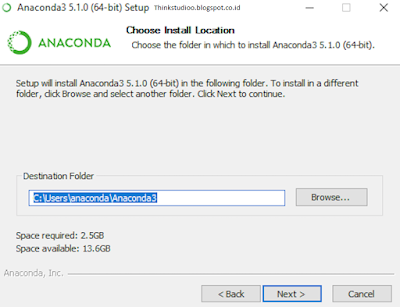
\includegraphics{1.png}
\caption{ Choose Install Location }
\label{1}
\end{figure}
\item
Lalu klik Next, kemudian pastikan ceklis bagian Register Anaconda lalu Klik Instal
\begin{figure}[!htbp]
\centering
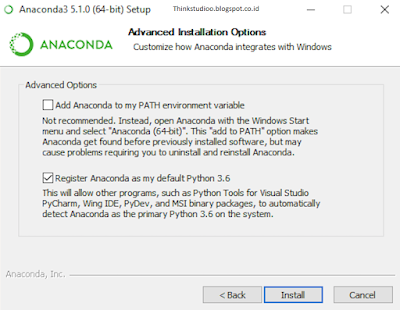
\includegraphics{2.png}
\caption{ Advance Installation Options }
\label{2}
\end{figure}
\item
Apabila belum menginstal Microsoft VS code, maka instal terlebih dahulu, apabila sudah, maka dapat di skip.
\begin{figure}[!htbp]
\centering
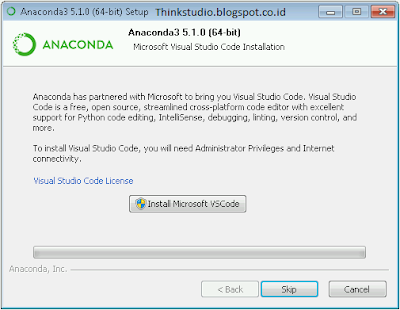
\includegraphics{3.png}
\caption{  }
\label{3}
\end{figure}
\item
Instalasi Selesai
\begin{figure}[!htbp]
\centering
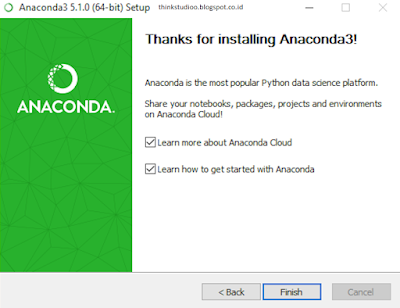
\includegraphics{4.png}
\caption{ Finish }
\label{4}
\end{figure}

\section{Cara Pemakaian Script dan Interpreter Python}
\subsection{Pemakaian Script dan Interpreter}
\begin{enumerate}
\item
Penulisan Statement
	Penulisan satu statement tidak diakhiri dengan tanda titik-koma. Apabila  menulis lebih dari satu statement dalam satu baris, maka harus memisahkannya dengan titik-koma.
Contoh :
print("Hello World!")
nama = "Tia"

\item
Penulisan String pada Python
	String dalam pemrograman ditulis dengan menggunakan tanda petik, menggunakan tanda petik tunggal maupun ganda.
Contoh:
judul = " Pemrograman Python "
penulis = 'Python'
Atau kita juga bisa menggunakan triple tanda petik.
Contoh:
judul = """Belajar Python """
penulis = '''Tia Nur Candida'''
\item
Penuilsan Case pada Python
	Sintak Python bersifat case sensitive.
Contoh:
judul = "Belajar Dasa-dasar Python"
Judul = "Belajar Membuat Program Python"
Variabel judul dengan Judul dibedakan.
\item
Penulisan Blok Program Python
	Blok program merupakan kumpulan dari beberpaa statement yang digabungkan dalam satu blok.
Penulisan blok program harus ditambahkan indentasi (tab atau spasi 2x/4x).
\item
Cara Penulisan Komentar pada Python
	Komentar merupakan baris kode yang tidak akan dieksekusi.
Komentar digunakan untuk memberikan informasi tambahan dan untuk menonaktifkan kode.
Ada beberapa cara menulis komentar pada pemrograman Python.
Menggunakan Tanda Pagar (#)
Cara pertama menggunakan tanda pagar (#).
Contohnya:
# ini adalah komentar
# Ini juga komentar
\item
Menggunakan Tanda Petik
Selain untuk mengapit teks (string), tanda petik juga dapat digunakan untuk membuat komentar.
Contoh:
"Ini adalah komentar dengan tanda petik ganda"
'Ini juga komentar, tapi dengan tanda petik tunggal'
Penulisan komentar dengan tanda petik jarang digunakan, kebanyakan orang lebih memilih untuk menggunakan tanda pagar. Jadi…tidak direkomendasikan.
\item
Menggunakan Triple Tanda Petik
Sedangkan triple tanda petik, sering digunakan untuk menuliskan dokumentasi.
\end{enumerate}

\subsection{Cara Pemakaian Spyder}
Cara Menggunakan:
\begin{enumerate}
\item
Admin Finder

php spyder.php http://situstarget –admin
\item
Auto Detect Cms

php spyder.php http://situstarget –cms
\item
Exploit Elfinder

php spyder.php http://situstarget/path/php/connector.php –exploit
\item
Scan Subdomain

php spyder.php http://situstarget –domain
\item
Scan Form Upload

php spyder.php http://situstarget –upload
\end{enumerate}
\section{Mencoba Python}
\begin{figure}[!htbp]
\centering
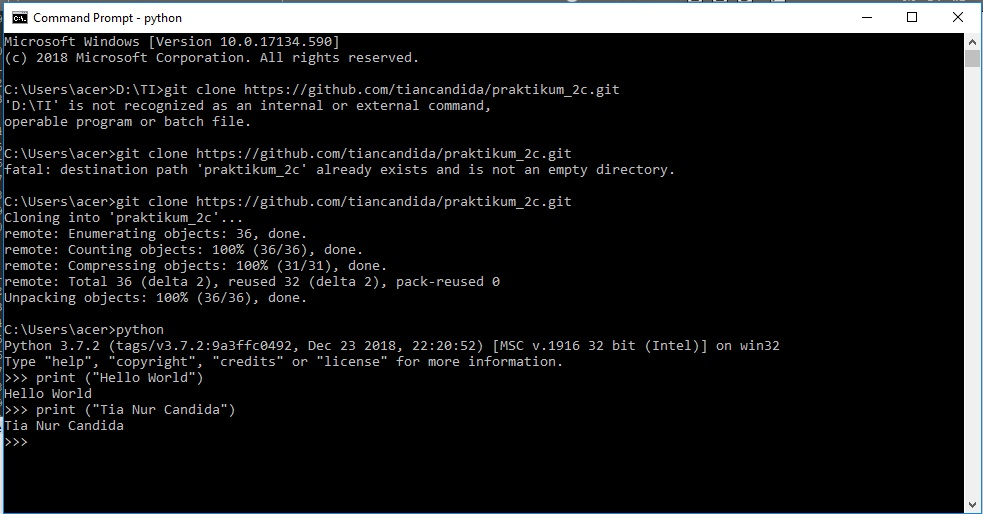
\includegraphics{hello world.jpg}
\caption{ Hello World }
\label{Hello World}
\end{figure}

\section{Identasi}
Python tidak menggunakan tanda { } untuk menandai blok atau grup kode. Blok kode di python menggunakan tanda indentasi (spasi). Jumlah spasi untuk setiap baris yang ada dalam satu blok kode harus sama.
Contoh :
if nilai <= 5:
   print("Nilai merah")
   print("Tidak lulus")
else:
   print("Nilai biru")
   print("Lulus")


\end{enumerate}
\end{document}